
\chapter{Optimization}\label{ch:optimization}

The optimization aims to find the model parameters $\theta$,
for which we minimize the loss function $\mathcal{L}(\hat{y}, y)$.
For this purpose, we calculate the gradient $\nabla_{\theta}\mathcal{L}(\hat{y}, y)$,
and iteratively update the parameters $\theta$ according to the optimization method, which in our case
is the \textit{Adaptive~Moment~Estimation} (\textit{Adam}) method~\cite{kingma2014}.
The \textit{Adam} method is the continuation of the iterative optimization method \textit{Stochastic~Gradient~Descent}
(\textit{SGD}), which averages both the gradient and the second moment of the gradient (Chapter~\nameref{ch:background}).

The optimization can be conceptually divided into two, closely related parts.
In the beginning, we present the process of model optimization.
We focus on two basic parameters in particular, the \textit{learning~rate} and the \textit{batch~size}.
Then in the next section, we present the essential system optimizations.
To perform a series of experiments in highly limited time is only possible
if the optimization process is adapted to the available infrastructure.
The efficient implementation of the system is crucial because
it allows doing experiments in a reasonable time.


\section{Model Optimization}\label{sec:model-optimization}

The optimization method is the \textit{Adam}, and the key parameters of the optimization method are
the \textit{batch size} and the \textit{learning rate} (Chapter~\nameref{ch:background}).
The forgetting factors for gradients and second moments of gradients, respectively, equals
$\beta_1=0.9$ and $\beta_2=0.999$.

\begin{figure}[h]
    \centering
    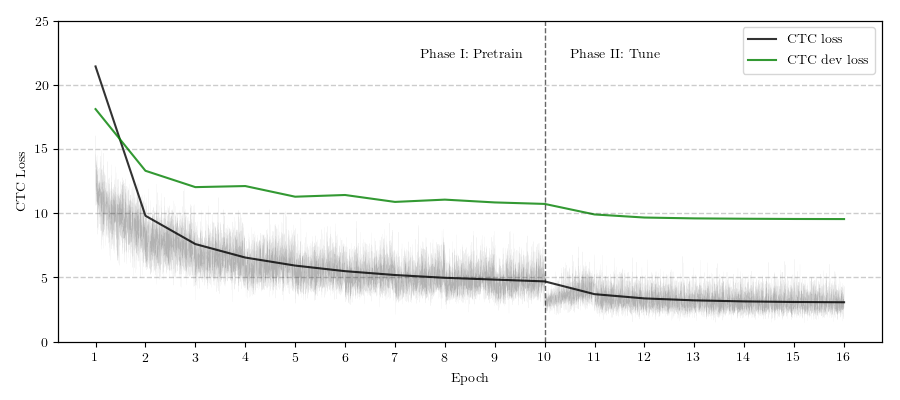
\includegraphics[width=0.9\textwidth]{figures/optimization-learning_rate.png}
    \caption{
The optimization process of the arbitrary model without an augmentation technique.
The optimization is divided into two phase: \textit{Pretrain} (left) and \textit{Tune} (right).
}
    \label{fig:learning_rate}
\end{figure}

The \textit{CTC~Loss} function tends to reach high values for longer utterances.
The high values of the loss function destabilize the training process at an early stage of optimization in particular.
Therefore for the first epoch, we sort samples by increasing length, as described in~\cite{amodei2015}.
However, in our case, this approach is not essential because samples are trimmed
up to 7 words (Chapter~\nameref{ch:data}).


\subsection*{Learning Rate}

Although the optimization method \textit{Adam} belongs to the \textit{adaptive~gradient~algorithm} group of methods,
the predefined \textit{learning rate} parameter $\eta$ still has the significant impact on the optimization process.
To define a priori the accurate learning rate $\eta$ is a tough task.
We do a set of initial experiments to define an appropriate learning rate scheduler, which
finally is composed of two phases.
In the first \textit{pretrain} phase, the learning rate is constant, and equals $\eta=10^{-3}$.
The relatively large learning rate aims to overcome a high \textit{plateau},
especially in the initial phase of optimization (the figure~\ref{fig:data_histograms}).

In the second \textit{tune} phase, the learning rate is reduced to $\eta=10^{-4}$
(samples once again are sorted), and is being reduced in subsequent epochs according to the equation:
\begin{equation} \label{eq:lr_scheduler}
\eta := \frac{\eta}{k^{epoch}}
\end{equation}
where $k=1.2$.
The second phase aims to fine-tune parameters in the discovered stable parameters region.
The presented learning rate scheduler is used unchangeable for each experiment.


\subsection*{Batch Size}

Most of the model optimizations converge with the \textit{mini batch} of size over 32 samples, where
the models that use the \textit{Batch~Normalization} regularization are an exception.
The \textit{Batch~Normalization} is based on the batch statistics~\cite{laurent2015}.
The statistics within a small batch are highly inaccurate, what in consequence, leads to the strong
model regularization, and in extreme cases causes the destabilization of training.
The optimization on the smallest possible convergent \textit{mini batch} leads to better results,
thanks to the vast number of iterations.
However, training is often difficult to perform due to high fluctuations and long plateaus.
On the other hand, a larger batch size significantly reduces the optimization time.
The computing \textit{GPU} units are used efficiently,
when the transmitted matrices for calculation are maximally large.
In consequence, as the trade-off, each model is optimized with a batch size equals 256 (reduced twice in relation to~\cite{amodei2015}).
It is worth noting that all samples in a single batch are aligned to the longest sample in a batch.
In case of very long utterances, the batch does not fit on the \textit{GPU} units, which unexpectedly results
in the critical error (\textit{Out Of Memory}) and stopping the calculations.
The problem disappears when the samples are trimmed.


\section{System Optimization}\label{sec:system-optimization}

The model optimization has to be adapted to the available infrastructure on which the calculations are performed.
We do the experiments on two identical computer clusters.
A single experiment uses the 5 \textit{graphical process units} (\textit{GPU}) with the 12 GB memory.\footnote{
The GPU units are the NVIDIA Tesla K80.
}
Furthermore, each machine has the 46 \textit{CPU} processors, used for the data preprocessing.
In this section, we outline the three system optimization techniques, which help to do experiments effectively.

It is worth noting that the optimization time strongly depends on the number of model parameters (figure~\ref{fig:time}).
The size of the model is one of the factors taken into consideration when exploring the different model architectures,
since working with larger models limits the number of experiments.

\begin{figure}[h]
    \centering
    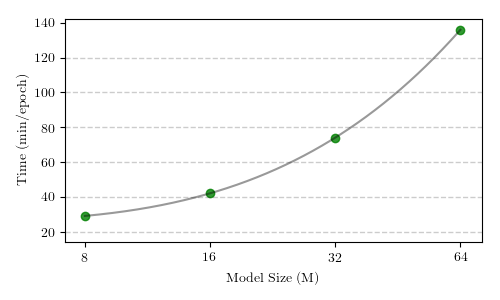
\includegraphics[width=0.6\textwidth]{figures/optimization-time.png}
    \caption{
The correlation between the duration of a single epoch and the size of the model (the first series of experiments~\ref{sec:base-model}).
}
    \label{fig:time}
\end{figure}


\subsection*{Features Preprocessing}

Firstly, we reduce the waiting time for the preparation input data as much as possible.
The preprocessing is done parallel to the model optimization and is carried out on parallel \textit{CPU} processes.
The prepared input batches are waiting in the queue (in the RAM).
Alternatively, the input data can be loaded from previously processed data, and saved in
the \textit{Hierarchical Data Frame} (\textit{HDF}) container~\cite{folk2011}.
The container is designed to read the stored data quickly, as well in parallel processes.


\subsection*{Data Parallelism}

The next step is to use efficiently the available \textit{GPU} units thanks to the \textit{data parallelism}.
The \textit{data parallelism} replicates the model to all GPUs, where each model
processes its input data portion independently.
Then the partial results from various GPUs are combined on CPU into one complete batch.
Our implementation allows for the quasi-linear acceleration on 5 GPUs.
However, the condition is to operate on relatively large batch sizes,
so that the memory of each unit is overloaded to the capacity limit.


\subsection*{CuDNN-LSTM}

The \textit{LSTM} layer optimization, which is the core component of the model, is computationally expensive.
In our models, the \textit{LSTM} layer is implemented in the \textit{CuDNN} library using the \textit{CUDA API}.
In consequence, the model training is 7 times faster than a standard implementation in the \textit{tensorflow} library~\cite{abadi2016}.
As a result, the computing cost against the basic \textit{RNN} layer has decreased, and the benefits of
using a \textit{LSTM} layer have become more apparent~\cite{amodei2015}.
